\documentclass{article}

\usepackage{graphicx}
\usepackage{tikz}
\usepackage{tikzsymbols}
\usetikzlibrary{calc,patterns,shapes.geometric}
\pagestyle{empty}
\usepackage[margin=0pt]{geometry}
\geometry{papersize={14in,12in}}

\def\centerarc[#1](#2)(#3:#4:#5){\draw[#1] ($(#2)+({#5*cos(#3)},{#5*sin(#3)})$) arc (#3:#4:#5);}

\begin{document}
	\begin{figure}
		\centering
		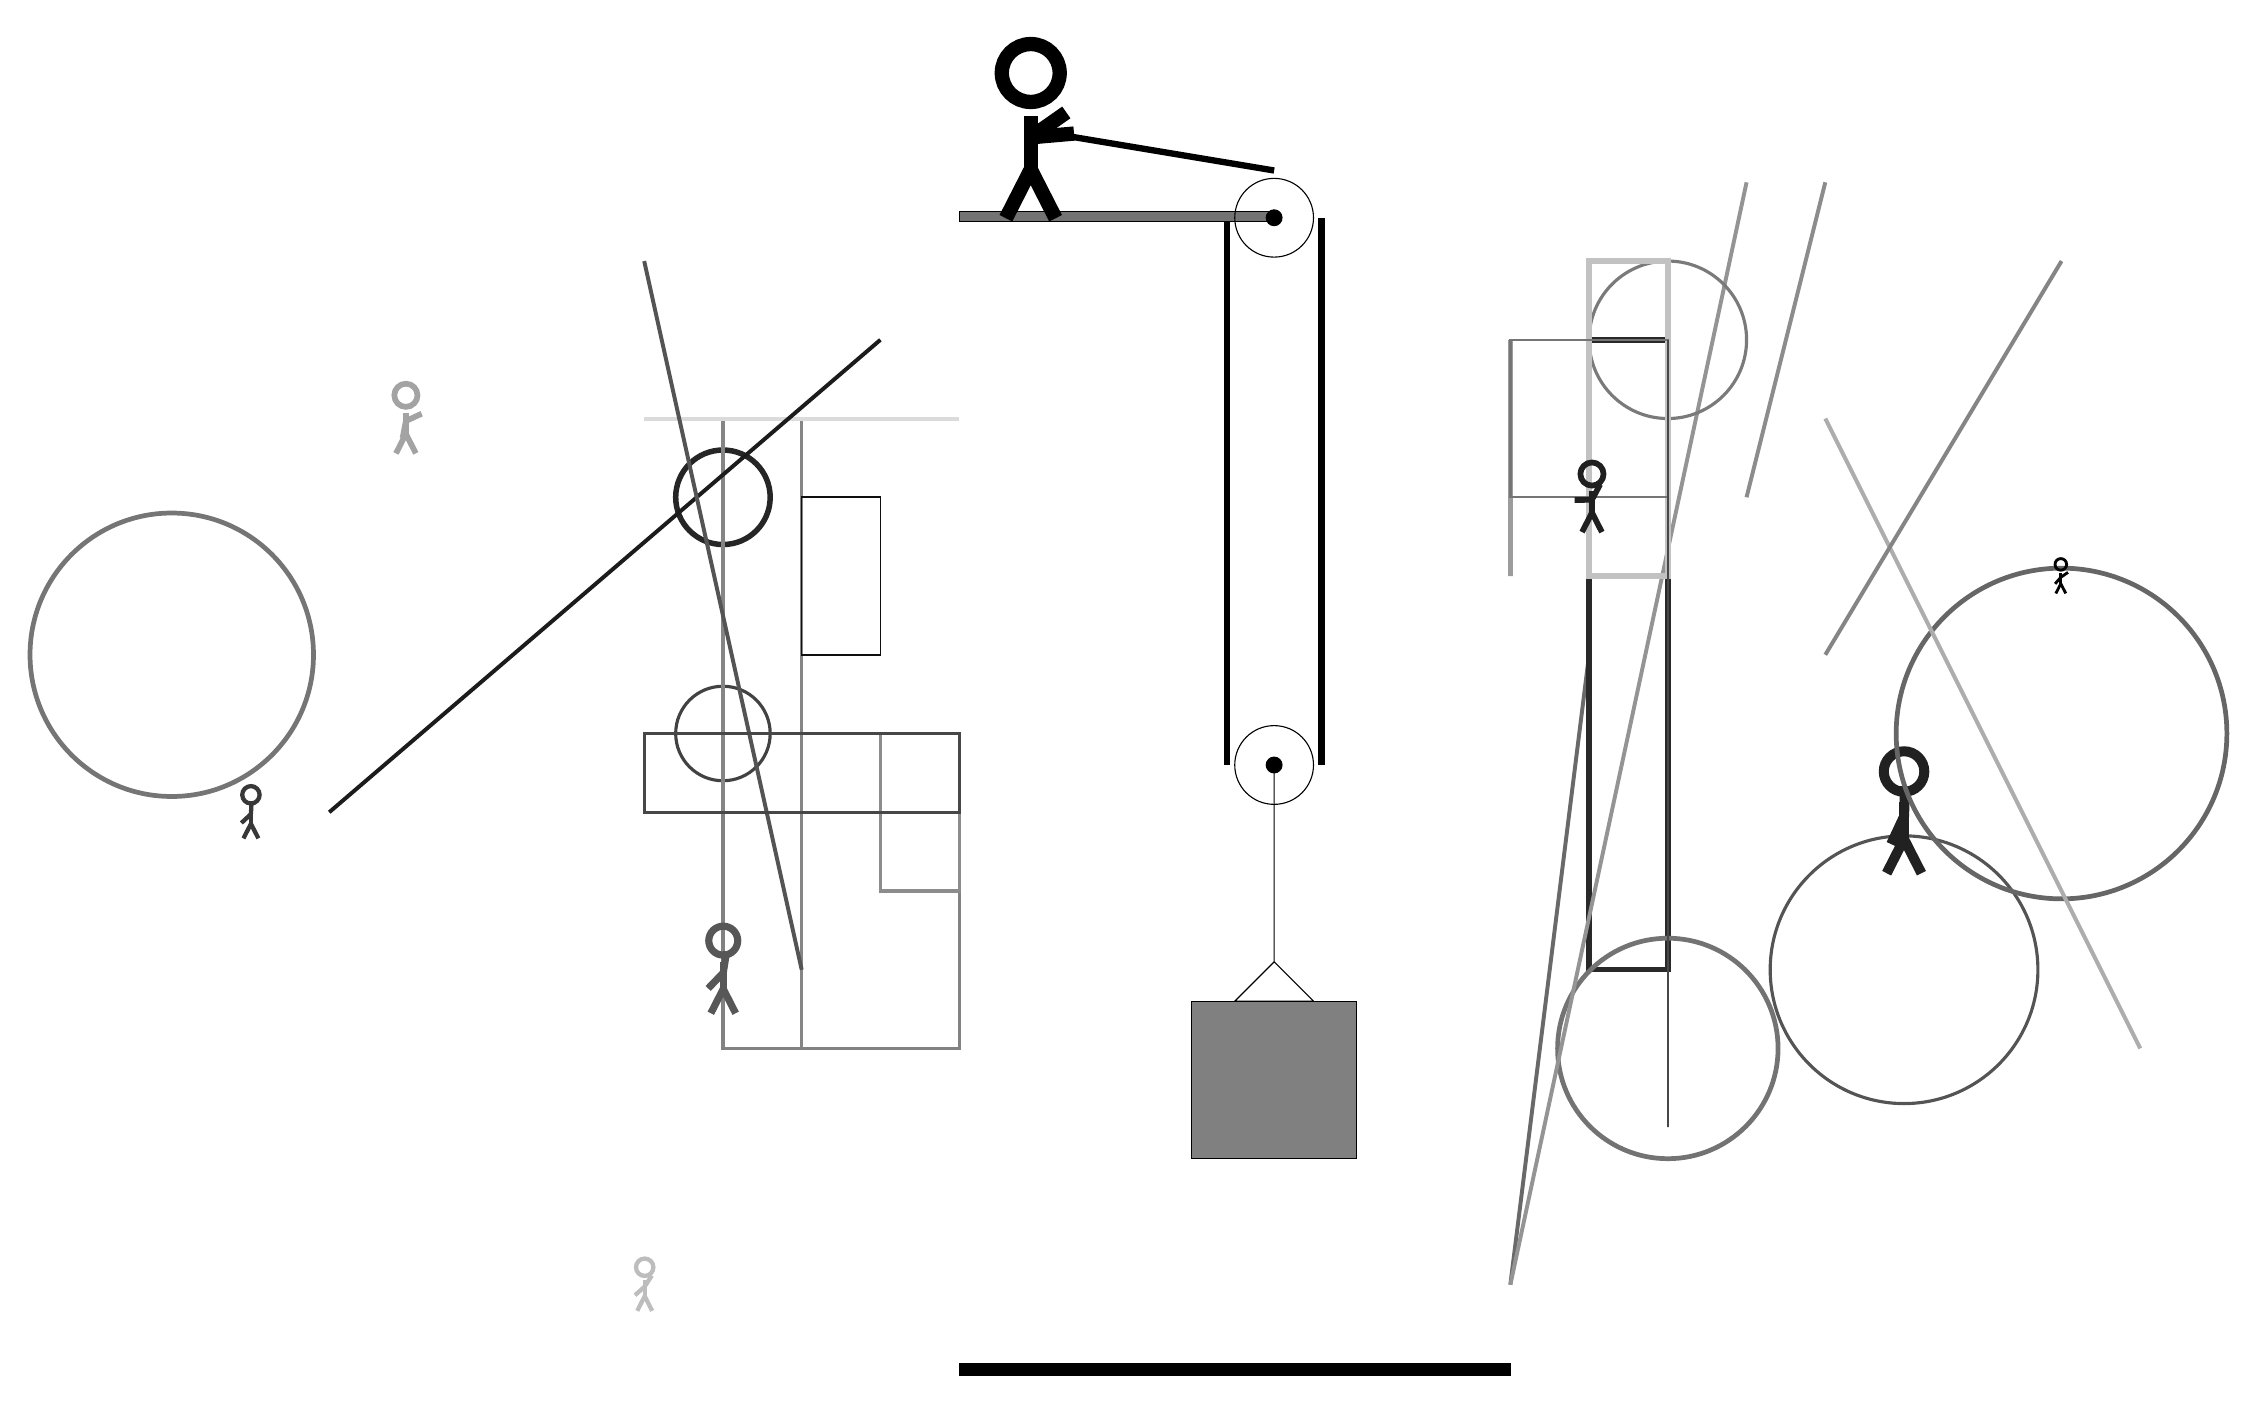
\begin{tikzpicture}
			%%%%% START %%%%%
			
			\draw[fill=black!55] (-2, 11.5) rectangle (2, 11.625);
			
			\draw (2, 4.6) circle (0.5);
			\draw[fill=black] (2, 4.6) circle (0.1);
			
			\draw (2, 11.55) circle (0.5);
			\draw[fill=black] (2, 11.55) circle (0.1);
			
			\draw (2, 4.6) -- (2, 2.1) -- (1.5, 1.6) -- (2.5, 1.6) -- (2, 2.1);
			\draw[fill=black!50] (0.95, 1.6) rectangle (3.05, -0.4);
			
			\draw[line width=0.8mm] (1.4, 11.5) -- (1.4, 4.6);
			\centerarc[line width=0.8mm](2, 4.6)(180:360:0.6);
			\draw[line width=0.8mm](2.6, 4.6) -- (2.6, 11.55);
			\centerarc[line width=0.8mm](2, 11.55)(0:90:0.6);
			\draw[line width=0.8mm](2, 12.15) -- (-1, 12.65);
			
			\node at (-1, 12.65) {\Strichmaxerl[10][-175][35]};
			
			\node[line width=0.7mm, color=black!78] at (-11, 4) {\Strichmaxerl[3][43][87]};
			
			\draw [line width=0.4mm, color=black!74](-5, 5) circle (0.6);
			\draw [line width=0.4mm, color=black!67](10, 2) circle (1.7);
			\draw[line width=0.5mm, color=black!59](6, 6) -- (5, -2);
			
			\draw[line width=0.7mm, color=black!84] (7, 2) rectangle (6, 10);
			
			\draw [line width=0.7mm, color=black!85](-5, 8) circle (0.6);
			
			\draw [line width=0.6mm, color=black!55](7, 1) circle (1.4);
			\draw[line width=0.5mm, color=black!42](5, -2) -- (8, 12);
			\node[line width=0.4mm, color=black!87] at (10, 4) {\Strichmaxerl[7][65][88]};
			\draw [line width=0.6mm, color=black!54](-12, 6) circle (1.8);
			
			\draw [line width=0.4mm, color=black!52](7, 10) circle (1.0);
			\draw [line width=0.6mm, color=black!60](12, 5) circle (2.1);
			\draw[line width=0.4mm, color=black!48] (-4, 9) rectangle (-5, 1);
			
			\draw[line width=0.7mm, color=black!39] (5, 10) rectangle (5, 7);
			\draw[line width=0.7mm, color=black!24] (6, 11) rectangle (7, 7);
			\draw[line width=0.5mm, color=black!55](-2, 9) -- (-3, 9);
			
			\draw[line width=0.4mm, color=black!49] (-2, 4) rectangle (-5, 1);
			\draw[line width=0.3mm, color=black!54] (5, 10) rectangle (7, 8);
			\draw [line width=0.5mm, color=black!63](-7, 9) circle (0.0);
			
			\draw[line width=0.5mm, color=black!32](9, 9) -- (13, 1);
			\node[line width=0.4mm, color=black!88] at (6, 8) {\Strichmaxerl[4][1][62]};
			
			\node[line width=0.7mm, color=black!99] at (12, 7) {\Strichmaxerl[2][49][34]};
			
			\draw[line width=0.5mm, color=black!14](-6, 9) -- (-2, 9);
			\node[line width=0.2mm, color=black!36] at (-9, 9) {\Strichmaxerl[4][79][25]};
			\draw[line width=0.5mm, color=black!45](8, 8) -- (9, 12);
			
			\draw[line width=0.2mm, color=black!72] (7, 10) rectangle (7, 0);
			
			\draw[line width=0.2mm, color=black!94] (-3, 8) rectangle (-4, 6);
			\draw[line width=0.4mm, color=black!45] (-2, 5) rectangle (-3, 3);
			\node[line width=0.5mm, color=black!66] at (-5, 2) {\Strichmaxerl[5][46][81]};
			
			\draw[line width=0.5mm, color=black!89](-3, 10) -- (-10, 4);
			\draw[line width=0.5mm, color=black!67](-6, 11) -- (-4, 2);
			
			\draw[line width=0.5mm, color=black!48](9, 6) -- (12, 11);
			\draw[line width=0.4mm, color=black!72] (-2, 4) rectangle (-6, 5);
			
			\node[line width=0.3mm, color=black!26] at (-6, -2) {\Strichmaxerl[3][42][57]};
			
			
			\draw[fill=black] (-2, -3) rectangle (5, -3.15);
			
			%%%%% END %%%%%
		\end{tikzpicture}
	\end{figure}	
\end{document}